\documentclass{standalone}
\usepackage{tikz}

\begin{document}



\tikzset{every picture/.style={line width=0.75pt}} %set default line width to 0.75pt

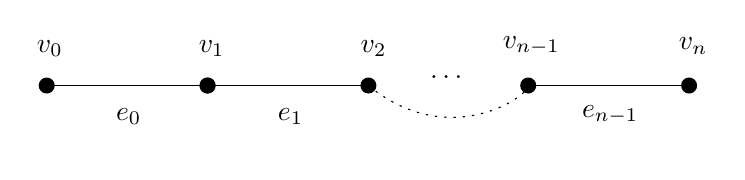
\begin{tikzpicture}[x=0.75pt,y=0.75pt,yscale=-1,xscale=1]
%uncomment if require: \path (0,462); %set diagram left start at 0, and has height of 462

%Straight Lines
\draw    (122.5,203) -- (200,203) ;
\draw [shift={(200,203)}, rotate = 0] [color={rgb, 255:red, 0; green, 0; blue, 0 }  ][fill={rgb, 255:red, 0; green, 0; blue, 0 }  ][line width=0.75]      (0, 0) circle [x radius= 3.35, y radius= 3.35]   ;
\draw [shift={(122.5,203)}, rotate = 0] [color={rgb, 255:red, 0; green, 0; blue, 0 }  ][fill={rgb, 255:red, 0; green, 0; blue, 0 }  ][line width=0.75]      (0, 0) circle [x radius= 3.35, y radius= 3.35]   ;
%Straight Lines
\draw    (200,203) -- (277.5,203) ;
\draw [shift={(277.5,203)}, rotate = 0] [color={rgb, 255:red, 0; green, 0; blue, 0 }  ][fill={rgb, 255:red, 0; green, 0; blue, 0 }  ][line width=0.75]      (0, 0) circle [x radius= 3.35, y radius= 3.35]   ;
\draw [shift={(200,203)}, rotate = 0] [color={rgb, 255:red, 0; green, 0; blue, 0 }  ][fill={rgb, 255:red, 0; green, 0; blue, 0 }  ][line width=0.75]      (0, 0) circle [x radius= 3.35, y radius= 3.35]   ;
%Straight Lines
\draw    (354.5,203) -- (432,203) ;
\draw [shift={(432,203)}, rotate = 0] [color={rgb, 255:red, 0; green, 0; blue, 0 }  ][fill={rgb, 255:red, 0; green, 0; blue, 0 }  ][line width=0.75]      (0, 0) circle [x radius= 3.35, y radius= 3.35]   ;
\draw [shift={(354.5,203)}, rotate = 0] [color={rgb, 255:red, 0; green, 0; blue, 0 }  ][fill={rgb, 255:red, 0; green, 0; blue, 0 }  ][line width=0.75]      (0, 0) circle [x radius= 3.35, y radius= 3.35]   ;
%Curve Lines
\draw  [dash pattern={on 0.84pt off 2.51pt}]  (277.5,203) .. controls (316.25,234.73) and (354.75,208.23) .. (354.5,203) ;



% Text Node
\draw (124,185) node [scale=1]  {$v_{0}$};
% Text Node
\draw (162,218) node [scale=1]  {$e_{0}$};
% Text Node
\draw (202,185) node [scale=1]  {$v_{1}$};
% Text Node
\draw (240,218) node [scale=1]  {$e_{1}$};
% Text Node
\draw (280,185) node [scale=1]  {$v_{2}$};
% Text Node
\draw (356,184) node [scale=1]  {$v_{n-1}$};
% Text Node
\draw (394,217) node [scale=1]  {$e_{n-1}$};
% Text Node
\draw (434,184) node [scale=1]  {$v_{n}$};
% Text Node
\draw (315,199) node   {$\ldots $};


\end{tikzpicture}

\end{document}
